
\documentclass[journal]{IEEEtran}
%
% If IEEEtran.cls has not been installed into the LaTeX system files,
% manually specify the path to it like:
% \documentclass[journal]{../sty/IEEEtran}

\hyphenation{op-tical net-works semi-conduc-tor}

\newcommand{\textot}[1]{\scalebox{0.95}{\texttt{#1}}}
\newcommand*{\equal}{=}

% graphs                                                          
%\usepackage{tikz}
%\usetikzlibrary{external}
%\tikzexternalize[prefix=tikz/]
%\usetikzlibrary{patterns}
\usepackage{pgfplots}
\usepackage{float}
\usepackage{graphicx}
\definecolor{green1}{HTML}{00BB00}
\definecolor{green2}{HTML}{66D666}
\definecolor{green3}{HTML}{B2EAB2}
\definecolor{blue1}{HTML}{0022AA}
\definecolor{blue2}{HTML}{0066CC}
\definecolor{blue3}{HTML}{99C1EA}
\definecolor{red0}{HTML}{E74C4C}
\definecolor{red1}{HTML}{DD0000}
\definecolor{red2}{HTML}{F19999}
\definecolor{yellow1}{HTML}{F1C239}
\definecolor{gray1}{gray}{0.9}
\definecolor{g}{RGB}{0, 150, 0}

% tables
%\usepackage{caption}
\usepackage{subcaption}
\usepackage{multirow}
\usepackage{booktabs}
\renewcommand\arraystretch{1.1}
\usepackage{amsmath}
\usepackage{arydshln}

% data
\usepackage{pgfplotstable}

% algorithms
\usepackage[ruled,vlined]{algorithm2e}
\usepackage{amsmath}
\usepackage{amsfonts}
\SetAlFnt{\footnotesize}
\SetKwInput{KwInit}{Initialization}
\setlength{\textfloatsep}{2pt}
\DeclareMathOperator*{\E}{\mathbb{E}}

\begin{document}
\title{Distributed Adaptive Rules with Apache Flink for Data Stream Mining -- Preliminary Work}

\author{Lukasz~Korycki, Virginia Commonwealth University, USA}%

\markboth{Journal of \LaTeX\ Class Files,~Vol.~14, No.~8, August~2015}%
{Shell \MakeLowercase{\textit{et al.}}: Bare Demo of IEEEtran.cls for IEEE Journals}

\maketitle

\begin{abstract}
	The abstract goes here.
\end{abstract}

% Note that keywords are not normally used for peerreview papers.
\begin{IEEEkeywords}
	IEEE, IEEEtran, journal, \LaTeX, paper, template.
\end{IEEEkeywords}

\IEEEpeerreviewmaketitle

\section{Introduction}

\IEEEPARstart{D}{ata} streams are infinite sources of knowledge and challenges. Sensors, web engines and monitoring systems generate countless data points every day and every second. On the one hand, we have unprecedented opportunities to analyze different phenomenas in a continuous and more adequate way -- not only from scare and incomplete snapshots, as it is in the case of off-line batch processing. On the other hand, we face several problems coming with the nature of rapid, dynamic and massive sources, that have to be properly addressed. 

In machine learning domain we have to take into consideration two substantial observations. Firstly, distributions of data streams are very often non-stationary. Concepts are evolving as time passes, unseen or rare data samples appears. We refer it as a concept drift. Secondly, streams are continuous and potentially infinite. There is no possibility of gathering the whole data and using it for a single batch-mode training. Processing of data streams is restricted to limited rationality, which means that quality and complexity of decisions made by streaming algorithms highly depend on finite computational resources. The algorithms are able to operate only on a partial and temporary knowledge. As a result, previously created models should be regularly adjusted to a dynamically changing environment, to evolving data streams.

The problem of keeping models up-to-date while working under strict constraints is the main concern of adaptive learning methods. In general, we can distinguish two groups of such algorithms: batch-based and on-line. The former may occur in a form of retraining or incremental updates. The latter is a special case of the incremental cases, with the restriction that each incoming instance has to be processed on-by-one, immediately and only once. It seems to be the most suitable to streaming data, since such methods tend to provide minimal latency and low memory occupations.

One of the main constraints is time -> distributed computing

In this work,

\section{Distributed adaptive rules}

While there are plenty of machine learning algorithms dedicated for data stream mining, like Hoeffding Trees [x] and Oza's ensembles [x], only few of them provide human-readable forms of models. This may be a significant problem in such domains as medicine or economy, in which automatic decisions should be properly explained.

\subsection{Rule-based models}
Rule-based algorithms and decision tress are the most suitable in such cases. While the latter are known to be very efficient in terms of computing time, the former is considered the most flexible due to modularity of decision rules.

One of the most popular classifiers based on rules is Adaptive Model Rules (AMR) proposed in [x]. It is an online model that incorporate knowledge from new instances by expanding its rules based on the widely used Hoeffding bound criterion [x]:

\begin{equation}
\label{eq:hbound}
\epsilon = \sqrt{\frac{R^2\ln(1/\delta)}{2n_l}},
\end{equation} 

\noindent where $R$ is a value range, $n_l$ is a number of examples seen on a node $l$ and $\delta$ is a confidence parameter. If a difference between two best attributes on the node is greater than $\epsilon$, then there is a $1-\delta$ confidence that the better attribute introduces superior information gain and it should be used to create a split.

While the flexibility and transparency of rule-based systems are their advantages, a high computational complexity is considered as one of the main drawbacks. Fortunately, since the models are modular, there is a lot of possibilities to improve their performance using parallelization techniques.

\subsection{Distributed computing}

One of the possible approaches is distribution of computations across several machines. The domain of distributed computing is currently occupied mainly by algorithms implemented in one of the three frameworks: Apache Spark, Flink or Storm. While all of them aim for increasing throughput of algorithms and decreasing latency in general, they are not suitable for all specific settings that may be distinguished in data stream mining.

\medskip
\begin{itemize}
	
	\item \textbf{Spark} -- it is highly oriented on batch processing and treats online processing as a special case of the former. The main idea behind this framework is to perform massive parallel computations on huge batches of data, so the overhead of scheduling tasks becomes minor. Originally, the main use case was to simply ensure computational feasibility for large data sets without a strong focus on the rate of incoming data. Currently, Spark has been evolving into a streaming framework with low latency of processing. Structured Streaming and Continuous Processing are two main features for such cases. The former is based on micro-batches of high-performing Data Frames, which decreases latency. However, since computation are still organized in batches, it may be prohibitive, for example, in cases with limited amount of labeled data Continuous processing enables strictly streaming processing, but since it is still in experimental mode, a lot of operators are not available yet. It is probably the main reason, why modeling online streaming processing is not very convenient in Spark at the moment. 
	\\
	\item \textbf{Flink} -- this framework can be somehow considered as opposite to Spark -- it is build around the idea of online processing, while batches are special cases of it. All operators in Flink are considered \textit{long-running}. It means that their instances (including parallel ones) are kept on tasks partitions constantly, so data literally \textit{flows} through them in a continuous stream from sources. Such approach naturally creates an environment for statefull computations in which parts of models are maintained in operator instances. It is especially important in the case of adaptive distributed machine learning algorithms.
	\\
	\item \textbf{Storm} -- it can be treated as a predecessor of Flink. Dedicated for online streaming processing, Storm organizes processing using spouts (sources) and bolts (operators), which handle streaming data. Currently, it seems that Storm is being gradually replaced with Spark Streaming and Flink. In addition, a low rate of contributions to its repository is an another factor that should be taken into consideration while choosing a framework.
	
\end{itemize}

\subsection{Distributed decision rules}
Due to the presented characteristics, it is not surprising that most of the streaming machine learning algorithms, even if few, have been implemented in Storm or Flink, mainly in SAMOA [x]. The already mentioned AMR algorithm is one of them [x]. 

There two main approaches to implementing this algorithm in a distributed manner. The first one is \textbf{vertical parallelization}, in which decision rules are distributed across several partitions, so all necessary updates are performed separately for each rule. Since there is still no efficient way to distribute prediction process without creating a synchronization barrier for each instance, in vertical architecture all conditions are maintained in a single rules aggregator, so only statistics for splits are distributed. One of the most important properties of this method, that should be emphasized, is that incoming instances does not wait for updates that arrive asynchronously.

The second approach is \textbf{horizontal parallelization}. In this architecture the algorithm maintains several independent rule models. It allows for processing several instances at the same time. Such approach definitely increases a throughput, however, since for each model a kind of subsampling is performed (depending on its availability), it also introduces a potential problem of undersampling. There is a third option (hybrid) that combines both approaches by introducing a common default rule, which propagates new rules to all models.

The AMR algorithm has already been implemented in Storm [x]. There is also an implementation of the Hoeffding Tree in Flink. However, to the best of our knowledge, AMR has not been integrated with the latter framework.

\section{Proposed implementations}

The proposed implementations of distributed adaptive rules in Flink are based on the original AMR and the two architectures mentioned in the previous section.

\subsection{Sequential}
The sequential version (\textot{SAMR}) of the algorithm's learning is almost the same as the original one [x]. For each incoming instance statistics are updated for all rules that covers it. If a sufficient number $N_{min}$ of instances was registered for a rule, the algorithm tries to expand the rule by looking for an attribute for which an effective split of classes can be established. For this purpose an entropy is calculated. If the value for the best possible split is significantly greater (Hoeffding bound) than a current rule's entropy, a new condition based on the split value is added to the rule and statistics are released.

If no rule covers and incoming instance, statistics for the default rule are updated and under the same circumstances, an expansion is attempted. If the rule received a condition, it is added to the set of maintained rules and a new default rule is created.

One of the crucial parts of the learning process is an approach to looking for the best split. The naive method that keeps the whole information about instances and analyzes possible bins sequentially, while calculating entropies, consumes a lot of time and memory. Some improvements are possible, like for example, utilizing a binary tree to optimize the searching [x]. However, to the best of our knowledge, the best solution, which can be also easily integrated with distributed architectures, is estimating the required class counters, using Gaussian distributions [x]. In such approach only a mean, standard deviation, counters, minimal and maximal attributes values have to be maintained. All of them can be calculated incrementally in an efficient way [x].

In the presented implementations, due to time limitations, we do not apply anomaly test nor removal of underperforming rules. This is the only different compared with the original algorithm, which, however, may be significant in the case of drifting data streams.

\subsection{Vertical parallelization}

In our vertical implementation (\textot{VAMR}) we used the following long-running operators, connections and data. We present only the most important elements. For more details, please, check the source code attached.

\medskip
\begin{itemize}
	\item[--] \textot{Rules Aggregator} -- it is a \textit{ProcessFunction} that receives instances as a main input. It performs all the operations (checking coverage, classification, maintaining the default rule) except for updates of rules statistics. Requests for the updates and initialization of new rules' statistics are sent, using a \textit{SideOutput}. The operator is placed in an iteration of \textit{IterativeStream} which allows for receiving a feedback from statistics partitions.\\
	
	\item[--] \textot{Partial Rules Processor} -- this parallel operator is responsible for updating statistics for given rules and expanding them. If a new condition is created, it is sent to the \textot{Rules Aggregator}. The number of these operators depends on a given level of parallelism (partitions).\\
	
	\item[--] \textot{Modulo Partitioner} -- it is responsible for distributing rule statistics between partitions. We simply use a modulo formula based on an rule's id.
\end{itemize}
\medskip

\begin{figure}[h]	
	\centering
	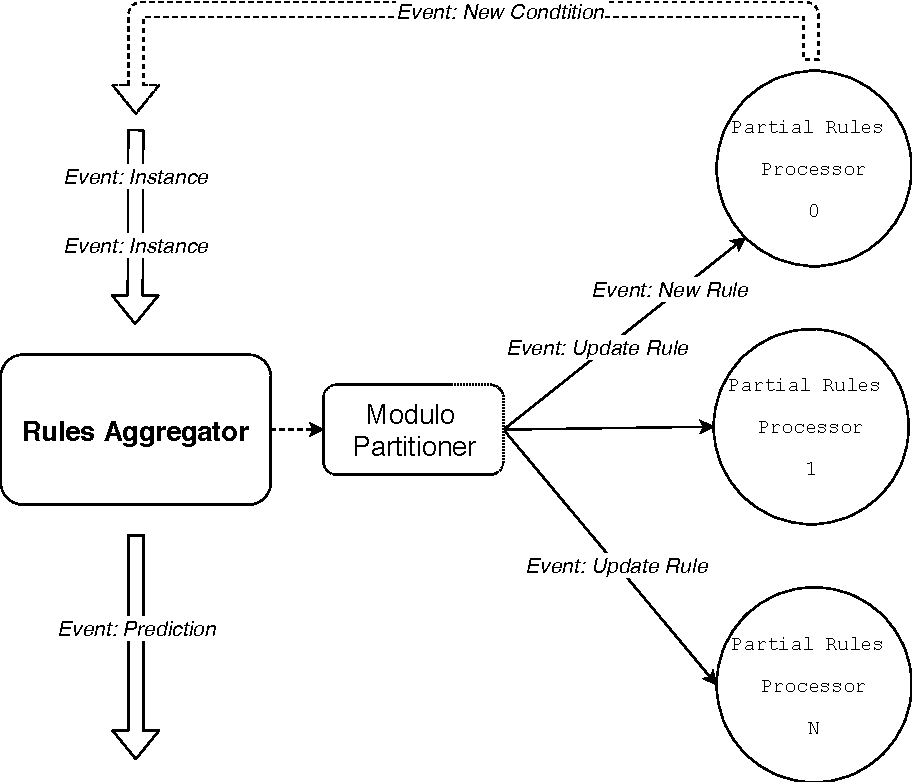
\includegraphics[scale=0.45]{img/vertical.pdf}	
	\caption{The vertical parallelization.}	
	\label{fig:vertical}
\end{figure}

\noindent Since different operators may receive different types od data, we needed to unify the data points into a common type, which is \textot{Event}.

\subsection{Horizontal parallelization}

To implement the horizontal parallelization (\textot{HAMR}) we simply created a pipeline connecting the input stream with \textot{Single Predictor}, which is a \textit{MapFunction} containing a single sequential model of ARM, and increased the number of partitions for it. As a result, we achieved our goal by utilizing basic Flink's capabilities.

\section{Experiments}

In the experimental section, we evaluated our implementations of the distributed AMR, using different data streams and levels of parallelism. We compared them with the sequential version of the algorithm.

\subsection{Data streams}

During the experiments, we used 10 different data streams (7 real and 3 synthetic). Most of them are supposed to be non-stationary. They are summarized in the Tab. \ref{tab:data}.

\begin{table}[h]
	\captionsetup{name=Tab}
	\caption{Summary of the used data streams.}
	\centering
	\scalebox{1.0}{\begin{tabular}[H]{m{1.25cm} >{\centering\arraybackslash} m{1.5cm} >{\centering\arraybackslash} m{1cm} >{\centering\arraybackslash} m{1cm} >{\centering\arraybackslash} m{1cm} >{\centering\arraybackslash} m{2.5cm}}	
			\toprule
			Name & Instances & Attributes & Classes & Type \\ 
			\midrule
			ActivityRaw & 1 048 570 & 3 & 6 & Real \\
			Connect4 & 67 557 & 42 & 3 & Real \\
			Covertype & 581 012 & 54 & 7 & Real \\
			Electricity & 45 312 & 8 & 2 & Real \\
			Hyperplane & 1 000 000 & 15 & 5 & Synthetic \\
			Lymph & 1 000 000 & 18 & 5 & Synthetic \\
			Olympic & 271 116 & 7 & 3 & Real \\
			Poker & 829 201 & 10 & 10 & Real \\
			Weather & 18 159 & 8 & 2 & Real \\
			Wine & 1 000 000 & 13 & 3 & Synthetic \\
			\bottomrule
			
	\end{tabular}}
	\label{tab:data}
\end{table}

\subsection{Set-up}

The experiments were conducted using 1, 2, 4 or 8 partitions on a local machine. We adjusted the minimum number $N_{min}$ of instances for expanding a rule, depending on a size of a stream (100 or 1000). The confidence parameter $\delta$ was equal to 0.05. For each setting we measured accuracy over a whole data stream, as well as time spent on computations.

\subsection{Results}

In this section, we present results of the described evaluation. In general, the AMR algorithm exhibited a mediocre performance (Tab. \ref{tab:acc_vertical}) with an exception for the Olympic stream (0.85) and Activity (0.32). The computing time (Tab. \ref{tab:time_horizontal}) varied significantly (standard deviation equal to about 42), which was caused by both data stream size and complexity of generated models.

\begin{table}[h]
	\captionsetup{name=Tab}
	\caption{Accuracy of SAMR and \textbf{relative accuracy} when running VAMR with different numbers of partitions P.}
	\centering
	\scalebox{1.0}{\begin{tabular}[H]{m{1.25cm} >{\centering\arraybackslash} m{1cm} | >{\centering\arraybackslash} m{1cm} >{\centering\arraybackslash} m{1cm} >{\centering\arraybackslash} m{1cm} >{\centering\arraybackslash} m{1cm} >{\centering\arraybackslash} m{1cm}}	
			\toprule
			Stream & SAMR & P=1 & P=2 & P=4 & P=8 \\ 
			\midrule
			Electricity & 0.7187 & 0.7154 & 0.6943 & 0.7180 & 0.6274\\
			Covertype & 0.6220 & 0.9590 & 0.8640 & 0.8524 & 0.9214\\
			Weather & 0.7008 & 0.9288 & 0.9793 & 0.9654 & 0.9793\\
			Activity & 0.3213 & 1.0459 & 1.0841 & 0.9470 & 1.1316\\
			Poker & 0.5548 & 0.8940 & 0.8694 & 0.9234 & 0.9355\\
			Olympic & 0.8527 & 0.9699 & 1.0007 & 0.9966 & 0.9924\\
			Hyperplane & 0.5822 & 1.0199 & 1.0096 & 1.0137 & 1.0228\\
			Wine & 0.6033 & 0.9106 & 0.9151 & 0.9036 & 0.9226\\
			Connect4 & 0.5618 & 0.9606 & 0.9310 & 1.0028 & 0.9976\\
			Lymph & 0.4900 & 1.0795 & 1.0637 & 1.0717 & 1.0853\\
			\midrule
			\textbf{Avg} & \textbf{0.6007} & \textbf{0.9484} & \textbf{0.9411} & \textbf{0.9394} & \textbf{0.9616}\\
			Std & 0.1423 & 0.1009 & 0.1145 & 0.0995 & 0.1358\\
			\bottomrule
			
	\end{tabular}}
	\label{tab:acc_vertical}
\end{table}

\begin{table}[h]
	\captionsetup{name=Tab}
	\caption{Computing time [s] for SAMR and \textbf{speed-up} when running VAMR with different numbers of partitions P.}
	\centering
	\scalebox{1.0}{\begin{tabular}[H]{m{1.25cm} >{\centering\arraybackslash} m{1cm} | >{\centering\arraybackslash} m{1cm} >{\centering\arraybackslash} m{1cm} >{\centering\arraybackslash} m{1cm} >{\centering\arraybackslash} m{1cm} >{\centering\arraybackslash} m{1cm}}	
			\toprule
			Stream & SAMR & P=1 & P=2 & P=4 & P=8 \\ 
			\midrule
			Electricity & 7.093 & 2.9070 & 3.9449 & 4.1946 & 4.0741\\
			Covertype & 24.453 & 1.0529 & 1.7989 & 2.3445 & 1.1923\\
			Weather & 1.854 & 1.6052 & 1.2493 & 1.0779 & 1.5725\\
			Activity & 57.101 & 2.3569 & 2.0596 & 2.6571 & 2.8897\\
			Poker & 29.076 & 2.7821 & 2.5237 & 0.9990 & 0.7239\\
			Olympic & 154.433 & 8.0104 & 11.9957 & 15.6103 & 18.7760\\
			Hyperplane & 56.423 & 2.5391 & 3.3036 & 5.2219 & 4.9093\\
			Wine & 26.612 & 1.0858 & 1.1218 & 0.9124 & 1.0133\\
			Connect4 & 7.37 & 0.7683 & 0.9750 & 0.9833 & 1.0824\\
			Lymph & 37.565 & 1.5611 & 1.6192 & 0.8845 & 1.4584\\
			\midrule
			\textbf{Avg} & \textbf{40.198} & \textbf{2.4669} & \textbf{3.0592} & \textbf{3.4886} & \textbf{3.7692}\\
			Std & 42.1967 & 2.0922 & 3.2834 & 4.5233 & 5.4596\\
			\bottomrule
			\\
	\end{tabular}}
	\label{tab:time_vertical}
\end{table}

One can see that the vertical parallelization leads to some drops in accuracy compared with SAMR, usually up to 0.1. The average drop was oscillating around 0.06 with a relatively high standard deviation (about 0.10), however, it was caused mainly by two data streams: Electricity (drop between 0.3-0.4) and Lymph (improvements about 0.07). At the same time, VAMR was able to provide a more less stable speedup between 3 and 3.5 for more than one partitions. However, it was elevated mainly by results for the Olympic stream (about 8-18), which also significantly increased variability of results. In most cases, the algorithm was not scaling up with the number of partitions. It was expected, since independent updates do not influence prediction in terms of the computing time. On the other hand, increasing the level of parallelization should positively influence accuracy (faster updates) -- it can be barely seen for P=8. It is possible that evaluation using a higher number of cores would provide more information about this relation. The speed-up observed for P=1 was a result of splitting prediction and updates into separate channels.

Much more encouraging results have been obtained for the horizontal parallelization. One can clearly see that HAMR was able to provide significant speed-ups (increasing more less directly proportionally to number of partitions for P=2 and P=4) while keeping accuracy on a similar level as SAMR. The average loss was about 0.01-0.02 with standard deviation between 0.02-0.08 that was increasing with the number of partitions, being elevated mainly by results for one data stream: Activity (1.05-1.18).

\begin{table}[h]
	\captionsetup{name=Tab}
	\caption{Accuracy of SAMR and \textbf{relative accuracy} when running HAMR with different numbers of partitions P.}
	\centering
	\scalebox{1.0}{\begin{tabular}[H]{m{1.25cm} >{\centering\arraybackslash} m{1cm} | >{\centering\arraybackslash} m{1cm} >{\centering\arraybackslash} m{1cm} >{\centering\arraybackslash} m{1cm} >{\centering\arraybackslash} m{1cm}}	
			\toprule
			Stream & SAMR & P=2 & P=4 & P=8 \\ 
			\midrule
			Electricity & 0.7187 & 0.9607 & 0.9248 & 0.8935\\
			Covertype & 0.6220 & 0.9702 & 0.9542 & 0.9034\\
			Weather & 0.7008 & 1.0013 & 1.0065 & 0.9891\\
			Activity & 0.3213 & 1.0539 & 1.1270 & 1.1849\\
			Poker & 0.5548 & 0.9682 & 0.9492 & 0.9326\\
			Olympic & 0.8527 & 1.0002 & 1.0003 & 0.9999\\
			Hyperplane & 0.5822 & 0.9828 & 0.9768 & 0.9564\\
			Wine & 0.6033 & 0.9924 & 0.9970 & 0.9474\\
			Connect4 & 0.5618 & 0.9835 & 0.9827 & 0.9930\\
			Lymph & 0.4900 & 1.0046 & 1.0038 & 1.0004\\
			\midrule
			\textbf{Avg} & \textbf{0.6007} & \textbf{0.9918} & \textbf{0.9922} & \textbf{0.9801}\\
			Std & 0.1423 & 0.0265 & 0.0545 & 0.0818\\
			\bottomrule
			
	\end{tabular}}
	\label{tab:acc_horizontal}
\end{table}

The algorithm was also able to slightly improve results in 3 other cases. It is an important observation, since it indicates that the ensemble of completely independent classifiers (regarding both training and prediction) may be sufficient enough while increasing throughput at the same time. To decide if the impact of such approach is meaningful, we would need to compare results with a single classifier that imply omit some instances.

\begin{table}[h]
	\captionsetup{name=Tab}
	\caption{Computing time [s] for SAMR and \textbf{speed-up} when running HAMR with different numbers of partitions P.}
	\centering
	\scalebox{1.0}{\begin{tabular}[H]{m{1.25cm} >{\centering\arraybackslash} m{1cm} | >{\centering\arraybackslash} m{1cm} >{\centering\arraybackslash} m{1cm} >{\centering\arraybackslash} m{1cm} >{\centering\arraybackslash} m{1cm}}	
			\toprule
			Stream & SAMR & P=2 & P=4 & P=8 \\ 
			\midrule
			Electricity & 7.093 & 2.2263 & 3.1595 & 4.7413\\
			Covertype & 24.453 & 1.7980 & 3.6410 & 3.7293\\
			Weather & 1.854 & 1.5593 & 1.7247 & 2.0108\\
			Activity & 57.101 & 1.7665 & 2.5766 & 7.2381\\
			Poker & 29.076 & 2.8361 & 5.0435 & 4.8452\\
			Olympic & 154.433 & 2.7139 & 5.8209 & 11.9373\\
			Hyperplane & 56.423 & 2.6296 & 8.2417 & 9.4369\\
			Wine & 26.612 & 2.7805 & 3.6236 & 4.0413\\
			Connect4 & 7.37 & 1.7370 & 2.7801 & 2.9899\\
			Lymph & 37.565 & 2.6975 & 3.5055 & 4.1176\\
			\midrule
			\textbf{Avg} & \textbf{40.198} & \textbf{2.2745} & \textbf{4.0117} & \textbf{5.5088}\\
			Std & 44.4792 & 0.5118 & 1.8947 & 3.1022\\
			\bottomrule
			\\
	\end{tabular}}
	\label{tab:time_horizontal}
\end{table}

Finally, we can conclude that the horizontal parallelization provides better relation between accuracy relative to the sequential algorithm and obtained speed-up. In Fig. \ref{fig:ratio} we can see that HAMR benefits from increased parallelization more that VAMR, since, as it was observed in the previous paragraphs, it keeps accuracy on a relatively stable level, while providing significant speed-up. It is possible that connecting both methods may lead to even further improvements [x].

\begin{figure}[h]
	\centering
		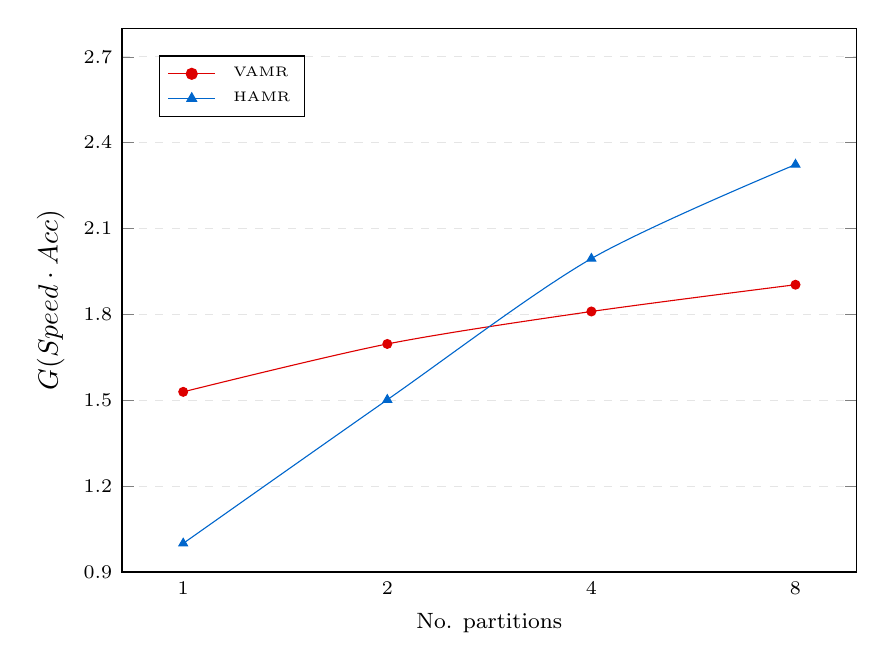
\begin{tikzpicture}
		\begin{axis}
		[
		title={},
		title style={yshift=-1.5ex},
		width=.9\columnwidth,
		height=.7\columnwidth,
		ymin=0.9,
		ymax=2.8,
		ytick={0.9,1.2,1.5,1.8,2.1,2.4,2.7},
		ymajorgrids=true,
		ylabel={$G(Speed\cdot Acc)$},
		ylabel near ticks,
		y tick label style={font=\scriptsize},
		extra y tick labels={},
		extra y tick style={
			ymajorgrids=true,
			ytick style={
				/pgfplots/major tick length=0pt,
			},
			grid style={
				gray,
				dashed,
				/pgfplots/on layer=axis foreground,
			},
		},
		grid style={dashed,white!90!black},
		xtick style={draw=none},
		xtick=data,
		xticklabels={1,2,4,8},
		xlabel={No. partitions},
		xlabel style={font=\footnotesize},
		x tick label style={font=\scriptsize},
		legend cell align={left},
		legend style={font=\tiny,column sep=1ex, legend columns=1, at={(0.05,0.95)}, anchor=north west},
		legend entries={VAMR,HAMR},
		]
		
		\addlegendimage{mark=*,red1,solid};
		\addlegendimage{mark=triangle*,blue2,solid};
		
		\addplot [	
		draw=red1,smooth,mark=*,mark options={red1,scale=0.8}
		] coordinates {(0,1.5295) (1,1.6968) (2,1.8103)	(3,1.9038)};
		
		\addplot [	
		draw=blue2,smooth,mark=triangle*,mark options={blue2,scale=0.9}
		] coordinates {(0,1.0000) (1,1.5019) (2,1.9951)	(3,2.3236)};
		
		\end{axis}
		
		\end{tikzpicture}
	
	\hspace*{0.4cm}
	\vspace*{-2mm}
	\caption{Geometric mean of speed-up (Speed) and relative accuracy (Acc) for VAMR and HAMR (P=1 is SAMR).}
	\label{fig:ratio}
\end{figure}

\section{Summary}


\begin{thebibliography}{1}
	
	\bibitem{IEEEhowto:kopka}
	H.~Kopka and P.~W. Daly, \emph{A Guide to \LaTeX}, 3rd~ed.\hskip 1em plus
	0.5em minus 0.4em\relax Harlow, England: Addison-Wesley, 1999.
	
\end{thebibliography}

\end{document}


